\documentclass[12pt]{article}
\usepackage{amsmath,amssymb,latexsym}
\usepackage{graphicx,psfrag,epsf}
\usepackage{enumerate}
\usepackage{natbib}
\usepackage{wrapfig}
\usepackage{subcaption}

\newcommand{\blind}{0}

\addtolength{\oddsidemargin}{-.75in}%
\addtolength{\evensidemargin}{-.75in}%
\addtolength{\textwidth}{1.5in}%
\addtolength{\textheight}{1.3in}%
\addtolength{\topmargin}{-.8in}%
\pagenumbering{gobble}

\begin{document}
\pagenumbering{arabic}

%\bibliographystyle{natbib}

\def\spacingset#1{\renewcommand{\baselinestretch}%
{#1}\small\normalsize} \spacingset{1}


%%%%%%%%%%%%%%%%%%%%%%%%%%%%%%%%%%%%%%%%%%%%%%%%%%%%%%%%%%%%%%%%%%%%%%%%%%%%%%

\if0\blind
{
  \title{\bf Refrigerator Based on the Throttling Effect }
  \author{Stanley Zheng \quad Yuzhe Wang}
  \maketitle
} \fi

\if1\blind
{
  \bigskip
  \bigskip
  \bigskip
  \begin{center}
    {\LARGE\bf Title}
\end{center}
  \medskip
} \fi

\bigskip
\begin{abstract}
Through this study of thermodynamics, we have learned about the throttling process. By utilizing the throttling process, we can create a small refrigerator without the need for a compressor. This report focuses on the creation of a refrigerator based on the throttling effect. As can be seen from the results, our refrigerator was able to achieve a cooling of 1.5 degrees Celsius.
\end{abstract}


\spacingset{1.45}
\section{Introduction}
\label{sec:intro}

The rapid development of human society has led to the widespread adoption of large appliances such as refrigerators in almost every household. Currently, the core component of most refrigerators available on the market is a compressor. In other words, these refrigerators are based on the principle that compressing a certain amount of gas produces heat while expanding it absorbs heat.

However, is it possible to create a refrigerator using alternative methods? The answer is yes. In this experiment, we employed a different principle, namely the throttling effect, to construct a refrigerator.

The throttling effect offers an alternative approach to refrigeration by harnessing the phenomenon of pressure reduction. By allowing a gas to pass through a narrow opening or throttle valve, a decrease in pressure occurs, resulting in a drop in temperature. This principle forms the basis of our experimental refrigerator design.

The objective of this study is to explore the feasibility and effectiveness of utilizing the throttling effect as a means of refrigeration. By investigating the performance of our refrigerator prototype, we aim to evaluate its cooling capabilities and compare them to conventional compressor-based refrigerators.

In this paper, we will present a detailed account of our experimental principle, procedure, and results. Through this research, we hope to shed light on the possibilities and limitations of employing the throttling effect as a viable approach to refrigerator design.


\section{Principle}


The basic idea of the refrigerator is the Throttling process, or isenthalpic process, in which the enthalpy remains constant. During the throttling process, the refrigerator does no work, and no heat is transferred from or to the refrigerator.

Under the isenthalpic process, the sum of the enthalpy from the part does not change.
$$
E_1 + P_1V_1=E_2+P_2V_2
$$

Then, the fan will form the airflow from $V_1$ to $V_2$, which increases $P_2$ and decreases $P_1$. We note that $V_1$ and $V_2$ remain constants so when $P_2$ increases and $P_1$ decreases, $E_2$ decreases and $E_1$ increase. Therefore, according to the relationship between internal energy and temperature, the temperature of $V_2$ will decrease.


\section{Experimental Procedure}

\begin{figure}[htb]
\centering
\subfloat[Actual Structure Diagram.]{
		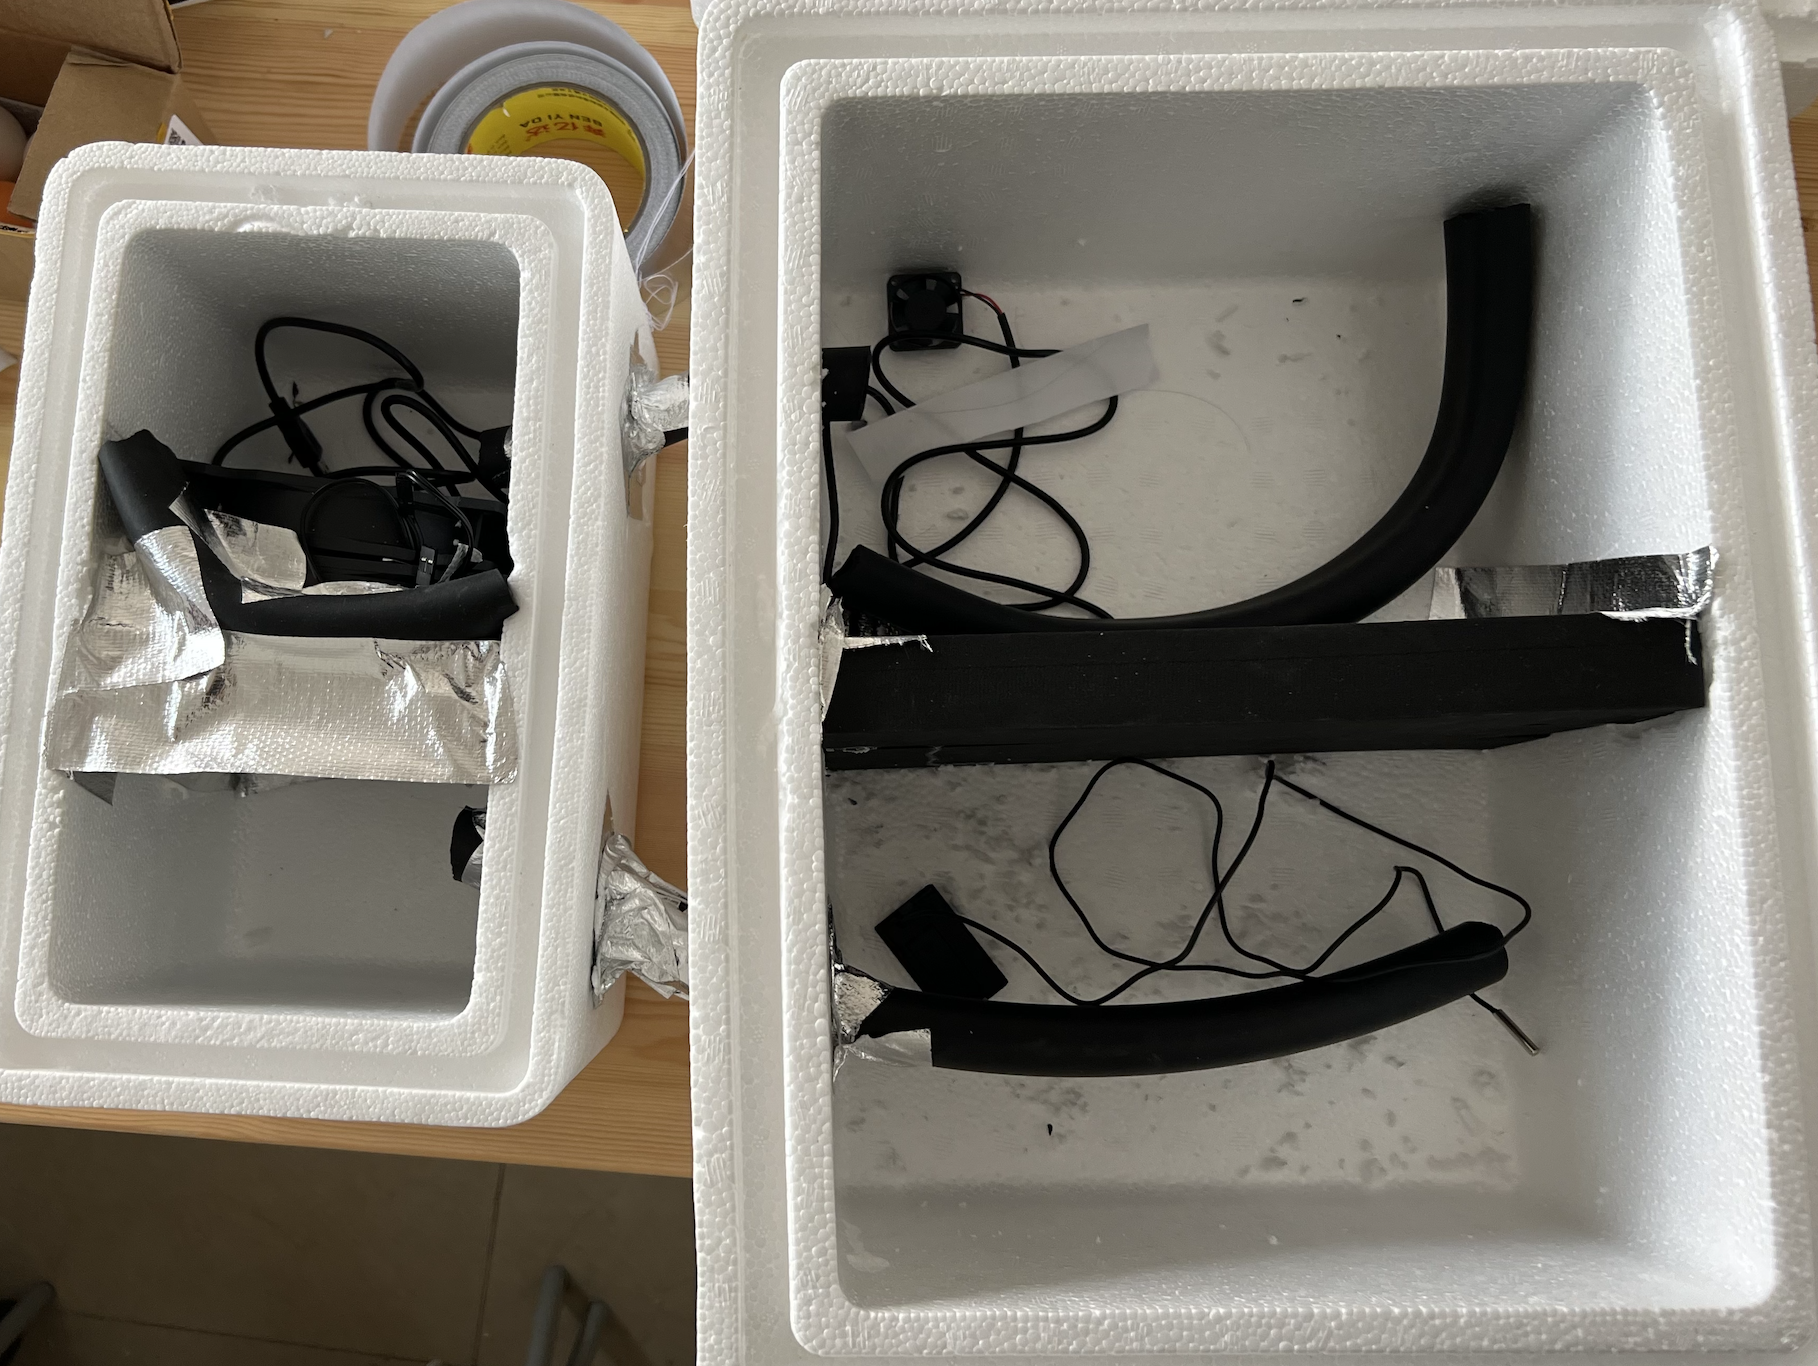
\includegraphics[scale=0.25]{3.png}}
\subfloat[Model Design Diagram.]{
		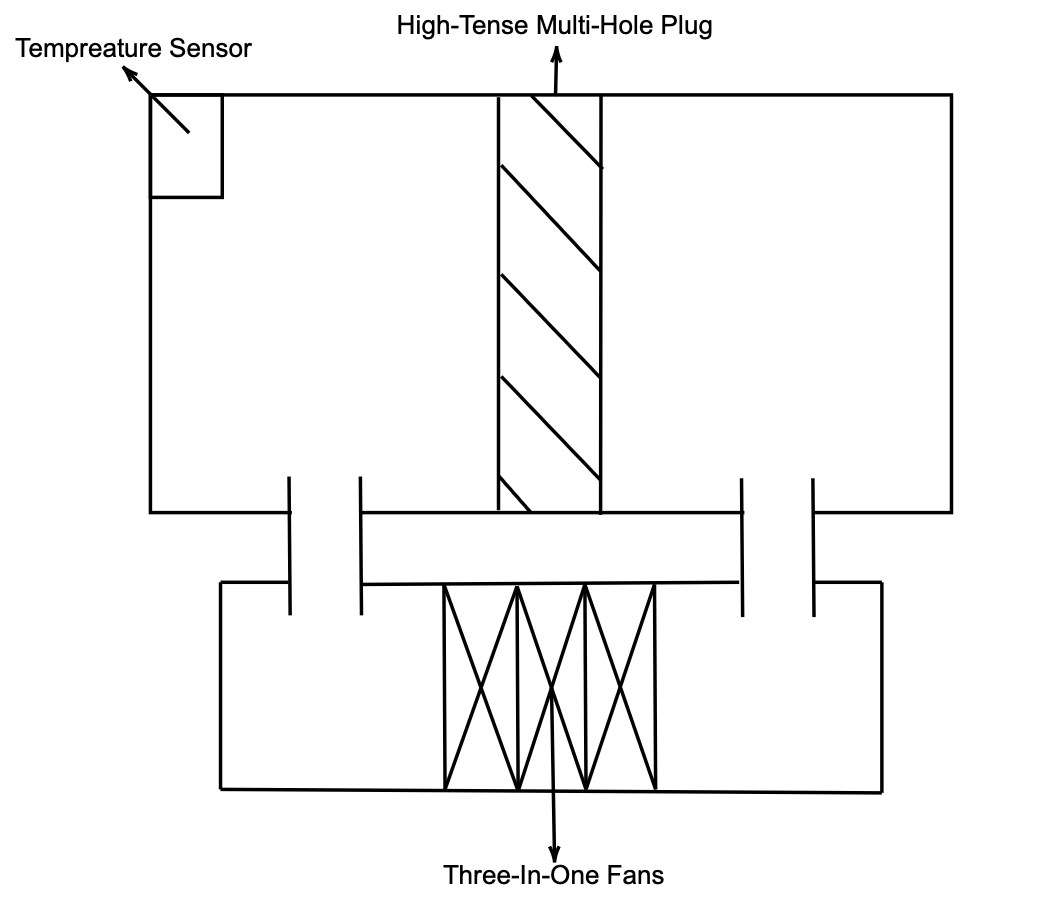
\includegraphics[scale=0.45]{1.png}}
\caption{Structure Diagram.}
\end{figure}

As the Figure 1 showns, our experimental setup consists of two insulated foam boxes, one serving as the windbox and the other as the refrigerator. We have a three-in-one fan, and two insulated hoses connecting the windbox and the refrigerator. Inside the refrigerator, there is a thick high-density sponge acting as a partition.
First, we measure the temperature inside the refrigerator. Then, we place the thermometer inside the refrigerator, close the lid, and turn on the fan. After two hours, we observe the reading on the thermometer inside the refrigerator.
\newpage

\section{Results}
We can see from the Figure 2 that initially the room temperature is $13.8^{\circ} $C.
\begin{figure}[htb]
\centering
\subfloat[Indoor Temperature.]{
		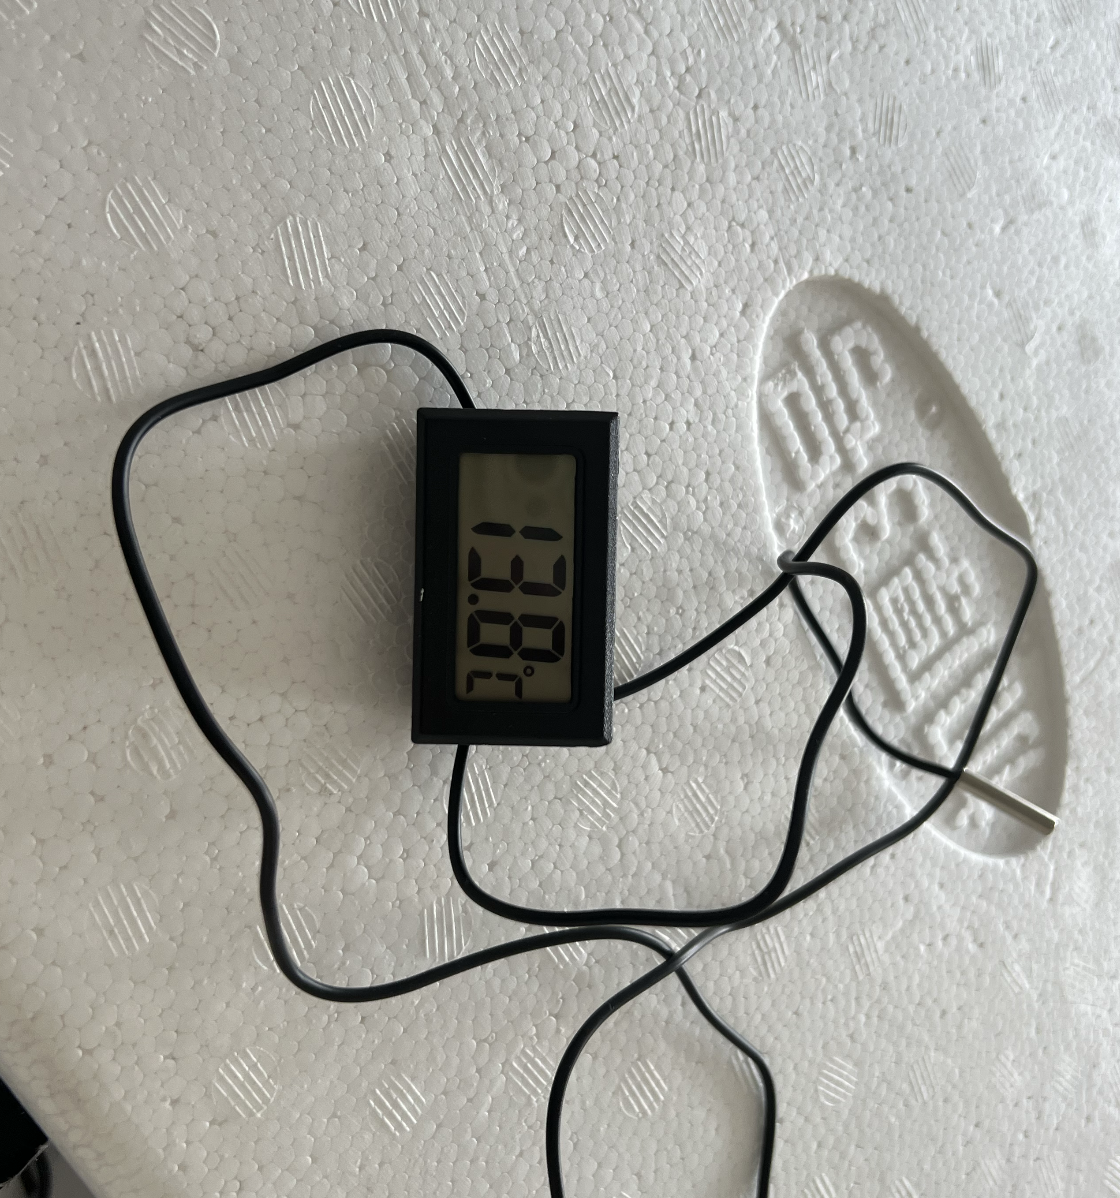
\includegraphics[scale=0.23]{4.png}}
\subfloat[Refrigerator Temperature.]{
		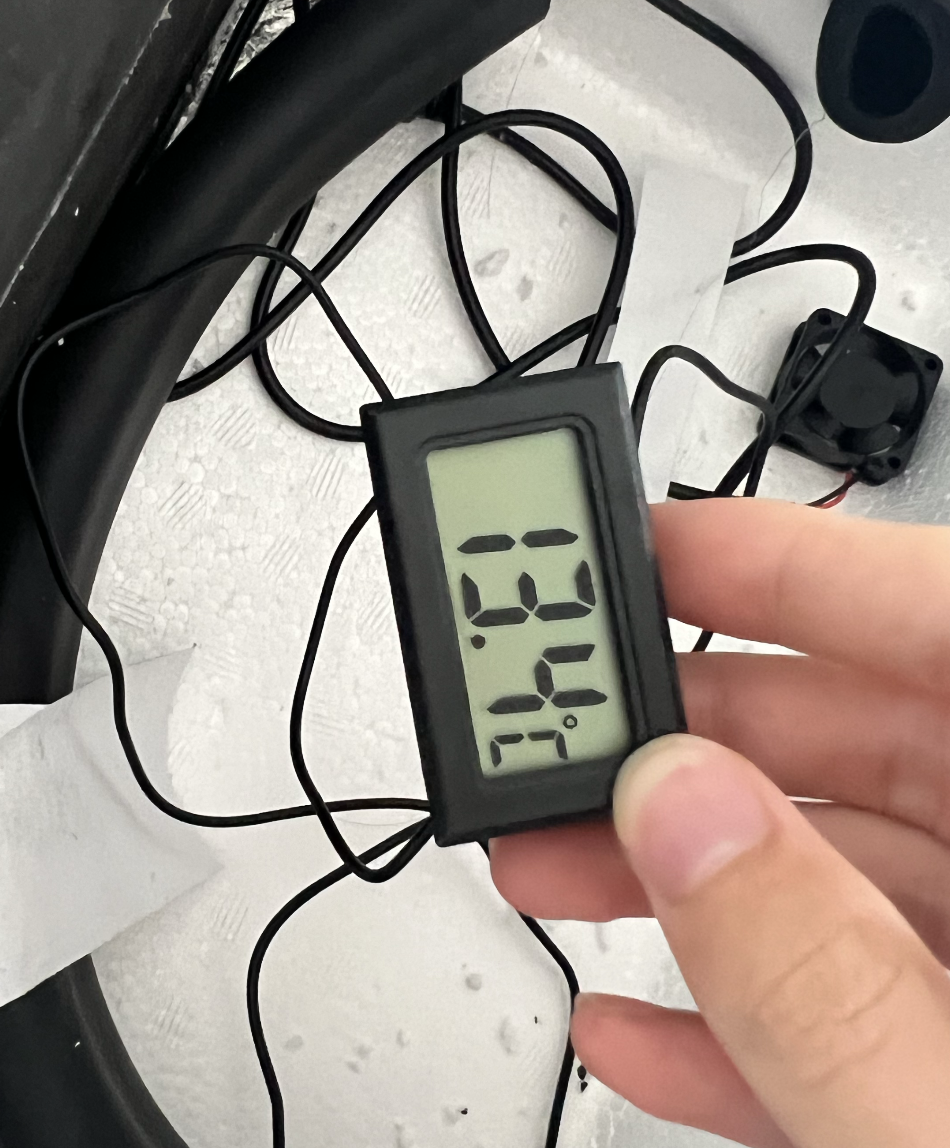
\includegraphics[scale=0.24]{5.png}}
\caption{Measured Temperature.}
\end{figure}

After a two-hour measurement, we obtained the temperature inside the refrigerator is $13.4^{\circ}$C.

It can be observed that the refrigerator does indeed have a certain cooling effect.

\section{Discussion}
\label{sec:con}
The key points of this experiment lie in maintaining a pressure difference across the insulated sponge and minimizing heat exchange that could affect the experimental results. There are many factors that can influence this, but the overall goal is to achieve a high level of sealing and insulation.

To achieve this, we used a large amount of insulated adhesive bags to wrap around all the joints, and all materials used were insulated.

Furthermore, according to the principle of throttling, we know that when the density of the sponge is sufficient, the fan blowing into the refrigerator must provide a strong enough airflow to maximize the pressure difference on both sides of the sponge and achieve the throttling effect. We used a powerful three-in-one fan to ensure an adequate airflow.

Our main innovation lies in the addition of a windbox. Without the windbox, it would be challenging to direct the airflow into the tubes, especially if we wanted to achieve precision by embedding the fan in the tube. Without embedding, it would be difficult to deliver the airflow effectively. By adding a windbox, we were able to maximize the input of sufficient airflow, provided we solved the connection issue with the windbox.

\end{document} 